%!TEX root=../Vorlage_DA.tex
%	########################################################
% 				Darstellung der Variablen
%	########################################################
\chapter{Darstellung der Variablen}

Die Anzeige der Variablen während der Laufzeit ist eine essentielle Funktion der Benutzeroberfläche. Die anschauliche und übersichtliche Darstellung soll dem Benutzer ein fundiertes Verständnis für den Ablauf des Programmes und die Rolle der Variablen darin, sowie deren Gültigkeitsbereiche vermitteln.

%	--------------------------------------------------------
% 	Unterschiede zu einem Debugger
%	--------------------------------------------------------
\section{Unterschiede zu einem herkömmlichen Debugger}
Die Idee der Variablendarstellung während der Laufzeit ist mit einem Debugger vergleichbar. Allerdings unterscheidet sich die Darstellung von Programmabläufen und Variablen in C Compact in einigen Punkten von herkömmlichen Debuggern:
\begin{itemize}
\item Während die Debugger professioneller Entwicklungsumgebungen eine Hilfestellung für erfahrene Programmierer sind, ist der Debugmodus von C Compact besonders auf Anfänger ausgelegt.
\item Die Darstellung der Variablen ist übersichtlich und fester Bestandteil der Beutzeroberfläche von C Compact. Einsteiger und unerfahrene Programmierer sollen von Anfang an mit dem Debugger in Berührung kommen.
\end{itemize}

%	--------------------------------------------------------
% 	Einführung + Erklärung Variablendarstellung
%	--------------------------------------------------------
\section{Darstellungsform der Variablen}

Zur Darstellung wurden zwei Konzepte verfolgt:
\begin{enumerate}
\item Die Anzeige des Call Stacks als Liste mit separaten Tabellen für die globalen und lokalen Variablen
\item Die Anordnung aller Variablen in einem Baum, wobei lokale Variablen Funktionen untergeordnet sind
\end{enumerate}

In den ersten Versionen der Benutzeroberfläche wurden die Variablen wie in Punkt 1 beschrieben dargestellt. Bereits während unseres Praktikums am Institut für Systemsoftware der JKU wurde die zweite Form der Variablendarstellung theoretisch entworfen. Die erste grundlegende Implementierung erfolgete noch während der Sommerferien.

In der ersten numerierten Version (Alpha 1.0) waren noch beide Darstellungsformen vorhanden und konnten vom Benutzer ausgewählt und gewechselt werden. Allerdings waren diese beiden Darstellungsformen sehr unterschiedlich implementiert, was Anfangs dazu führte, dass die Darstellung der Variablen als Baum nicht mehr als ein zusätzliches Feature ohne den vollen Funktionsumfang der Variablendarstellung als Call Stack war.

Für die Version Alpha 1.1 sollte ursprünglich das Variablendarstellungssystem so verändert werden, dass beide Anzeigemodi über ein gemeinsames Interface angesprochen werden können. Nach ausführlicher Besprechung und Evaluierung der unterschiedlichen Variablendarstellungen haben wir aber beschlossen, die Variablen nur als Baum darzustellen. Dadurch haben sich folgende Vorteile ergeben:
\begin{enumerate}
\item Die Implementierung einer neuen Funktion in der Variablenanzeige muss nur noch einmal erfolgen und nicht für jeden Anzeigemodus extra vorgenommen werden.
\item Daraus resultiert auch ein durchdachteres und einfacheres Bedienungskonzept der Benutezroberfläche, da dieses nur an eine Variablendarstellung angepasst werden muss.
\item Davon profitiert zuletzt der Benutzer, der eine komplette und sauber implementierte Anzeige und Erklärung der Variablen während des Programmablaufes vorfindet.
\end{enumerate}

%	--------------------------------------------------------
% 	Darstellung in getrennten Tabellen
%	--------------------------------------------------------
\section{Darstellung der Variablen in getrennten Tabellen}

Diese Form der Variablendarstellung wurde erstmals im Dokument Ausführungsumgebung für C-- von Herrn Professor Blachek beschrieben und nach dieser Vorlage implementiert\footnote{Ausführungsumgebung für C––, Günther Blaschek, V1.0, 2014-06-18}. Ein Vorteil dieser Darstellungsform war die Übersichtlichkeit und Einfachheit besonders beim Debuggen von einfachen Programmen. Leider verlor das Konzept an Übersichtlichkeit, wenn fortgeschrittene Programme mit komplexen Strukturen abgearbeitet wurden. Eine Tabelle konnte jeweils nur eine Ebene der Variablen, also beispielsweise den Inhalt einer Struktur oder die lokalen Variablen einer Funktion anzeigen.
\begin{figure}
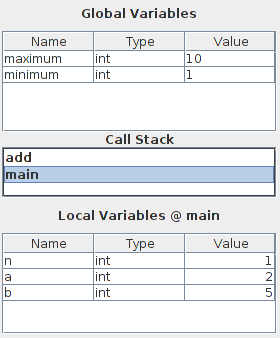
\includegraphics[width=8cm]{./media/images/gui/var/callstack.png}
\caption{Darstellung der Variablen in separaten Tabellen}
\label{var_sep}
\end{figure}

%	--------------------------------------------------------
% 	Darstellung als Baum
%	--------------------------------------------------------
\section{Darstellung der Variablen als Baum}

\subsection{Darstellungsschema}

Die Darstellung der Variablen in Form einer Baumstruktur hat den Vorteil, dass alle Variablen in einem Feld untergrbracht sind und die Gültigkeitsbereiche der Variablen sofort ersichtlich sind.
Alle Elemente befinden sich in einem Ordner, der den Namen der Datei trägt. Dadurch wird symbolisiert, dass die Variablen ein Teil des Programmes sind. Dem Programm selbst untergeordnet sind globale Variablen und Funktionen. Lokale Variablen sind Funktionen untergeordnet, Variablen in Strukturen sind der Struktur untergeordnet.
Zusätzlich werden folgende Elemente in der Tabelle farbig markiert:
\begin{itemize}
\item Funktionen sind hellblau hinterlegt. Sie sollen dadurch optisch von Datenstrukturen und Variablen unterscheidbar sein.
\item Die Variablen, die zuletzt geändert wurden, sind gelb hinterlegt. Grundsätzlich kann pro Schritt des Debuggers nur eine Variable geändert werden. Werden aber einige Schritte übersprungen, zum Beispiel mit dem Schlüsselwort \glqq library\grqq, so werden mehrere Variablen in einem Debuggerschritt geändert.
% TODO refer to library
\item Variablen, die noch nicht initialisiert wurden, sind grau hinterlegt.
% TODO refer to undef variables
\end{itemize}

\begin{figure}
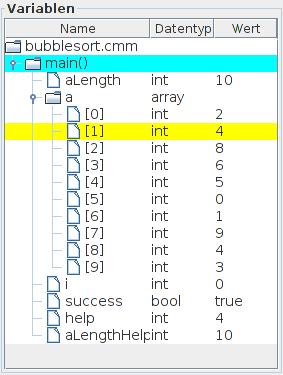
\includegraphics[width=8cm]{./media/images/gui/var/treetable.png}
\caption{Darstellung der Variablen als Baum}
\end{figure}

Bei Rechtsklick auf eine Variable im Baum wird ein Kontextmenü geöffnet. Mit der Option ,,Jump to declaration'' kann der Benutzer zur Deklaration der Variable im Sourcecode springen. Die entsprechende Zeile wird markiert.
% TODO jump to call???

\subsection{Grundlegende Komponenten}
Die Variablen werden in einer Tabelle mit Baumstruktur, in Kommentaren im Sourcecode deshalb oft ,,TreeTable'' genannt, angezeigt. Die TreeTable ist eine Kombination aus einem JTree und einer JTable.
Im Folgenden werden diese Komponenten beschrieben und der Aufbau der TreeTable erläutert:

\subsubsection*{JTree - Baum}
Ein JTree\footnote{http://www.codejava.net/java-se/swing/jtree-basic-tutorial-and-examples} ist Swing-Element, das Daten hierarchisch untereinander darstellet. Die Daten sind allerdings nicht im JTree selbst gespeichert, sondern in externen Objekten. Ein JTree kann entweder mit einem Datenmodell oder mit dem Hauptknoten eines Baumes initialisiert werden\footnote{http://docs.oracle.com/javase/tutorial/uiswing/components/tree.html}. Da die Daten eines JTree einen Baum abbildet, kann durch diese Struktur traversiert werden. Solche Operationen\footnote{http://www.java-tutorial.ch/core-java-tutorial/expande-or-collapse-all-nodes-in-a-jtree} werden beispielsweise benötigt, um alle Knoten eines Baumes zu öffnen (expand) oder zu schließen (collapse).
Wird ein JTree direkt mit einem Baum initialisiert, müssen die Knoten das Interface TreeNode implementieren\footnote{http://docs.oracle.com/javase/7/docs/api/javax/swing/tree/TreeNode.html}. Für einfache Aufgaben können Standardklassen, wie etwa DefaultMutableTreeNode\footnote{https://docs.oracle.com/javase/7/docs/api/javax/swing/tree/DefaultMutableTreeNode.html} verwendet werden.
Mehr Möglichkeiten bietet aber die explizite Verwedung eines Datenmodells. Ein Datenmodell regelt die Interaktion des JTree mit seinem Datenbaum und stellt Methoden zum Einfügen, Löschen und Ändern von Knoten sowie zum Auslesen des Pfades eines Knotens zur Verfügung.
Der JTree in der TreeTable von C Compact verwendet ein eigenes Datenmodell, TreeTableDataModel. Der Baum besteht aus Objekten der Klasse DataNode. Da ein eigenes Datenmodell verwendet wird, muss DataNode das Interface TreeNode nicht implementieren.

\subsubsection*{JTable - Tabelle}
Tabellen können in Swing mit dem Komponenten JTable\footnote{http://docs.oracle.com/javase/tutorial/uiswing/components/table.html} dargestellt werden. Wie auch bei der Klasse JTree werden die Daten nicht im Objekt von JTable gespeichert. Im einfachsten Fall kann eine Tabelle durch ein zweidimensionales Array initialisiert werden\footnote{http://www.java2s.com/Tutorial/Java/0240\_\_Swing/CreatingaJTable.htm}. In der Regel wird aber ein Datenmodell wie etwa DefaultTableModel\footnote{http://docs.oracle.com/javase/8/docs/api/javax/swing/table/DefaultTableModel.html} verwendet. Ein für eine Tabelle verwendbares Datenmodell ist ein Objekt einer Klasse, die das Interface TableModel\footnote{http://docs.oracle.com/javase/8/docs/api/javax/swing/table/TableModel.html} implementiert.

\subsection{Implementierung}
Die grundlegende Implementierung erfolgte anhand eines Blogeintrages\footnote{http://www.hameister.org/JavaSwingTreeTable.html}, mittlerweile wurde der Code allerdings stark an die Anforderungen der Benutzeroberfläche angepasst und erweitert.

Im folgenden Klassendiagramm wird der Aufbau der TreeTable dargestellt. Swing-Komponenten sind Dunkelblau, von Java vorgegebene Klassen und Interfaces sind Hellblau dargestellt. Die meisten Klassen sind selbst implementiert und daher mit weiß gekennzeichnet.

\begin{figure}
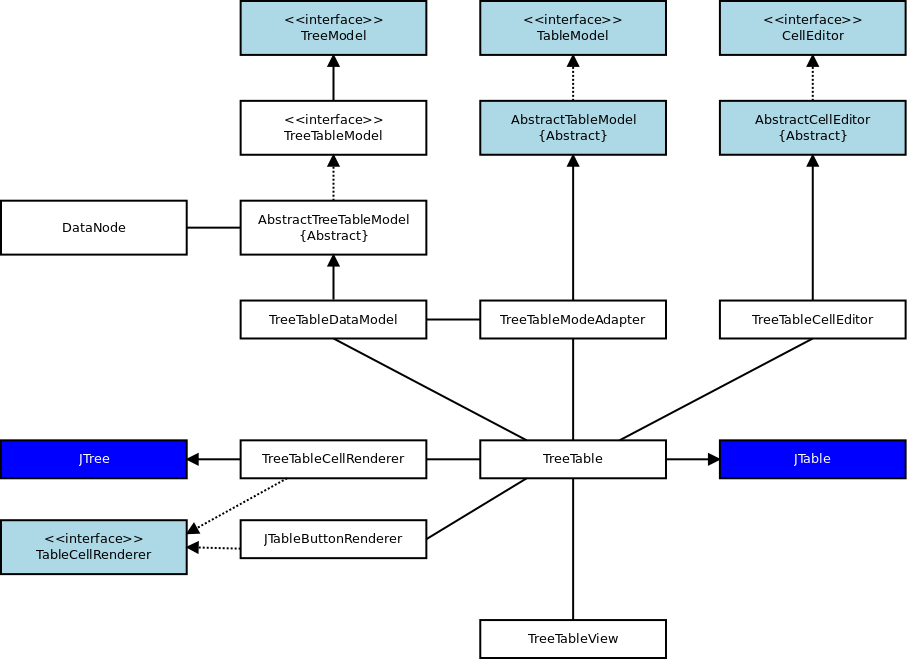
\includegraphics[width=\textwidth]{./media/images/gui/var/TreeTableClasses.png}
\caption{Klassendiagramm der TreeTable}
\label{var_tt_class}
\end{figure}

\subsubsection*{TreeTable.java}
Diese Klasse ist die Hauptklasse der TreeTable und, da sie von JTable erbt, eine Swing-Komponente. Hier laufen alle Teile der TreeTable, wie etwa Datenmodelle und Renderer, zusammen.

\subsubsection*{VarTreeTable.java}
VarTreeTable ist eine Wrapperklasse für TreeTable. Sie übernimmt alle wichtigen Funktionen zur Kommunikation mit dem Variablenbaum und bildet so eine Schicht zwischen dem Debugger und der TreeTable. Auf diese Weise wird der Code übersichtlicher und ist besser strukturiert.
TreeTableView hat folgende Methoden:
\begin{itemize}
\item \textbf{init} Initialisiert die TreeTable mit einem Standard-Datenmodell. Dieses besteht nur aus einem Hauptknoten (root), der den Namen der aktuellen Datei trägt; es werden keine Variablen angezeigt. Das Standard-Datenmodell wird immer dann angezeigt, wenn der Debugger nicht aktiv ist, also wenn der Benutzer den Sourcecode editiert.
\item \textbf{standby} Löscht das aktuelle Datenmodell und übergibt ein Standard-Datenmodell an die TreeTable, sodass wie zu Beginn nur der aktuelle Dateiname angezeigt wird. Diese Methode wird immer aufgerufen, wenn der Debugger beendet wird.
\item \textbf{update} Aktualisiert das Datenmodell der TreeTable im Debugmodus und zeigt die Variablen im Speicher des Interpreters an.
\item \textbf{highlightVariable} Mit dieser Methode wird die Addresse einer zuletzt geänderten Variable an die TreeTable übergeben. Diese Variable wird in der Tabelle markiert. Es ist möglich, diese Funktion mehrmals aufzurufen und so mehrere Variablen zu markieren. Wenn das Datenmodell mit \textbf{update} aktualisiert wird, verfallen alle Addressen.
\item \textbf{updateFontSize} Bei Aufruf dieser Methode wird die Schriftgröße der Tabelle geändert und die gesamte TreeTable neu gezeichnet. Diese Methode wird aufgerufen, wenn die Einstellungen der Benutzeroberfläche geändert wurden.
\end{itemize}

\subsubsection*{TreeModel.java}
TreeModel ist ein Interface für alle Datenmodelle eines JTree.

\subsubsection*{TreeTableModel.java}
Dieses Interface erweitert das Interface TreeModel so, dass es mit einer TreeTable kompatibel wird. TreeTableModel definiert zusätzliche Methoden, die für das Datenmodell einer Tabelle benötigt werden, beispielsweise ,,getColumnName()''.

\subsubsection*{AbstractTreeTableModel.java}
Diese abstrakte Basisklasse implementiert einige konkrete Methoden für die Verwendung als Datenmodell eines JTree. In Objekten dieser Klasse werden der Hauptnoten (root) des Baumes gespeichert. Außerdem regelt AbstractTreeModel den Ablauf von Änderungsevents in der Datenstruktur des Baumes.

\subsubsection*{DataNode.java}
Ein Datenknoten (DataNode) ist ein Knoten des in der TreeTable abgebildeten Baumes. In diesen Knoten sind alle nötigen Informationen zu den angezeigten Variablen - auch jene, die nicht im Baum selbst sondern in der Tabelle angezeigt werden - gespeichert.
\newline
Die Klasse DataNode hat folgende Felder:
\begin{lstlisting}[language=JAVA]
// Informationen, die in der Tabelle angezeigt werden
private final String name;
private Object type;
private Object value;

// Zusätzliche Informationen
private int address;
private int declaration;
\end{lstlisting}
Die TreeTable besitzt drei Spalten: In der ersten befindet sich der Baum mit den Namen der Variablen. in der zweiten Spalte wird der Datentyp der Variable und in der dritten ihr Wert gezeigt. Die Felder für Datentyp und Wert haben den Typ Object, da sich in der Tabelle an der Stelle eines Wertes auch ein JButton befinden kann.
%TODO refer to JTableButtonRenderer.java
Zusätzlich werden die Addresse und die Deklarationszeile der Variable gespeichert. Die Adresse dient der eindeutigen Identifikation der Variable, zum Beispiel beim Traversieren durch den Variablenbaum. Dadurch können lokale Variablen auch bei mehrfachem Aufruf einer Funktion unterschieden werden.
Bei Rechtsklick auf eine Variable in der TreeTable wird ein Kontextmenü mit der Option ''Jump to declaration'' geöffnet. Im Sourcecode wird dann die Zeile markiert, die im Feld ''declaration'' des betreffenden Datenknoten gespeichert ist.

\subsubsection*{TreeTableDataModel.java}
TreeTableDataModel erbt von AbstractTreeTableModel beinhaltet einen weiteren Schritt zu einem Tabellen-Datenmodell. Beispielsweise sind Methoden implementiert, die im Datenmodell einer Tabelle benötigt werden. Außerdem wird in dieser Klasse das kontrete Aussehen der Tabelle festgelegt, indem die Tabellenspalten definiert sind:
\begin{lstlisting}[language=JAVA]
// Column names
static protected String[] columnNames = {_("Name"), _("Type"), _("Value")};
 
// Column types
static protected Class<?>[] columnTypes = {TreeTableModel.class, String.class, Object.class};
\end{lstlisting}

\subsubsection*{TableModel.java}
Dieses Interface bildet die Grundlage für alle Datenmodelle einer JTable\footnote{http://docs.oracle.com/javase/7/docs/api/javax/swing/table/TableModel.html}.

\subsubsection*{AbstractTableModel.java}
In dieser abstrakten Basisklasse sind bereits die meisten Methoden des Interface TreeModel implementiert\footnote{http://docs.oracle.com/javase/7/docs/api/javax/swing/table/AbstractTableModel.html}. Der Benutzer muss lediglich die folgenden Methoden selbst definieren:
\begin{lstlisting}[language=JAVA]
public int getRowCount();
public int getColumnCount();
public Object getValueAt(int row, int column);
\end{lstlisting}
Diese Methoden werden in der Klasse TreeTableModelAdapter implementiert.

\subsubsection*{TreeTableModelAdapter.java}
TreeTableModelAdapter bildet die Verbindung zwischen dem Datenmodell der Tabelle und dem des Baumes. Diese Klasse erbt von AbstractTreeTableModel und enthält eine Referenz auf TreeTableDataModel. Viele Methoden, wie etwa ,,getColumnName()'' oder ,,getValueAt()'' sind in TreeTableDataModel implementiert, da sich in dieser Klasse auch das eigentliche Datenmodell der TreeTable befindet, und werden in TreeTableModelAdapter übernommen. Beispielsweise greifen die folgenden Methoden auf die Implementierung in TreeTableDataModel zurück:
\begin{lstlisting}[language=JAVA]
public Object getValueAt(int row, int column) {
   return treeTableModel.getValueAt(nodeForRow(row), column);
}

public boolean isCellEditable(int row, int column) {
   return treeTableModel.isCellEditable(nodeForRow(row), column);
}
\end{lstlisting}

\subsubsection*{CellEditor.java}
Dieses Interface bildet die Grundlage für alle Klassen, die CellEditor einer JTable sind\footnote{https://docs.oracle.com/javase/7/docs/api/javax/swing/CellEditor.html}.
Ein CellEditor ist für die Dateneingabe in eine Tabelle verantwortlich\footnote{http://docs.oracle.com/javase/tutorial/uiswing/components/table.html\#editor}. Die einfachse Form eines CellEditors ist ein DefaultCellEditor\footnote{https://docs.oracle.com/javase/7/docs/api/javax/swing/DefaultCellEditor.html}. Dieser unterstützt die Eingabe von Daten in die Tabelle mithilfe eines Textfeldes, einer Checkbox oder einer Combobox.

\subsubsection*{AbstractCellEditor.java}
AbstractCellEditor ist eine abstrakte Basisklasse für alle Arten eines CellEditor in Swing\footnote{https://docs.oracle.com/javase/7/docs/api/javax/swing/AbstractCellEditor.html}. Einige grundlegende Methoden sind bereits implementiert.

\subsubsection*{TreeTableCellEditor.java}
Daten in der TreeTable sollen vom Benutzer zwar nicht verändert werden können, wenn das Editieren der Tabelle mit der Methode ,,setEditable()'' aber deaktiviert wird, werden auch Events (wie etwa Mausklicks) nicht mehr registriert. TreeTableCellEditor gibt also Events in der Tabelle bei Bedarf an den JTree weiter und verbietet Events in Zellen, die nur Text enthalten.

\subsubsection*{TableCellRenderer.java}
In diesem Interface sind alle Methoden definiert, die zum Rendern von Zellen einer JTable benötigt werden\footnote{https://docs.oracle.com/javase/7/docs/api/javax/swing/table/TableCellRenderer.html}.

\subsubsection*{TreeTableCellRenderer.java}
Diese Klasse erbt von JTree und wird verwendet, um einen Baum in die erste Spalte der Treetable zu rendern. Außerdem ist diese Klasse dafür verantwortlich, dass die Zeilen der Tabelle und des Baumes die selbe Höhe haben und dass die Zellen die richtige Farbe erhalten.
%TODO refer to table line colors

\subsubsection*{TableButtonRenderer.java}
Diese Klasse wird als Renderer für die zweite und dritte Spalte der TreeTable verwendet. Sie erlaubt das Verwenden von Swing-Komponenten wie etwa JButtons als Zellendaten und sorgt dafür, dass die Zellen die korrekte Hintergrundfarbe haben.

%TODO weitere Elemente der TreeTable: Popup, Kontextmenü

